\section{Sprint 5: Refactor del proyecto y consolidación del generador}
\label{sec:refactor-consolidacion-generador}

Una vez realizadas las primeras pruebas del generador, el código del fichero 
\textbf{project\_generator.py} había crecido considerablemente hasta convertirse 
en un módulo difícil de mantener y depurar. Esta situación causó un refactor 
profundo del proyecto, que no se limitó al generador sino que abarcó también 
los ficheros de presentación, el sistema de prompts y la trazabilidad de las 
llamadas al LLM.

Este sprint se dividió en dos bloques principales. En primer lugar, la 
refactorización del generador y de los ficheros de presentación, dividiendo 
el código en módulos más pequeños y mantenibles. En segundo lugar, la 
incorporación de nuevas funcionalidades de trazabilidad y análisis, como el 
modelo \textbf{GenerationLog}, el verificador de consistencia y el panel de 
métricas.

\subsection{Refactor del generador en módulos}
\label{subsec:refactor-generador-modulos}

Estos cambios fueron muy importantes, los pasos del generador se realizaban con 
todo el contenido dentro del mismo fichero, algo que no era de fácil escalabilidad 
a futuro, por lo que el primer cambio fue dividir el \textbf{project\_generator.py} 
en cuatro ficheros encargados cada uno de una labor especifica dentro de 
\textbf{utils/generator}, como se muestra en la Figura~\ref{fig:modulos-generador}.

\begin{figure}[H]
    \centering
    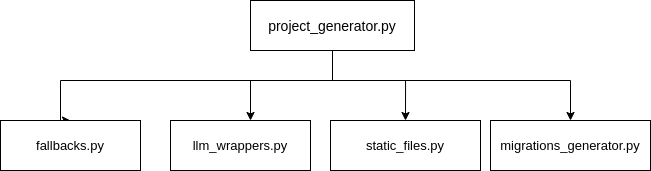
\includegraphics[width=0.8\textwidth]{img/disenoimplementacion/modulosgenerador}
    \caption{Estructura de módulos del generador tras el refactor}
    \label{fig:modulos-generador}
\end{figure}

\begin{itemize}
    \item \textbf{\texttt{llm\_wrappers.py}}: Centralizó todas las llamadas 
    al LLM en tres funciones reutilizables. \texttt{llm\_call} para llamadas 
    básicas que devuelven texto, \texttt{llm\_json\_call} para llamadas que 
    esperan JSON como respuesta, y \texttt{llm\_call\_logged} para llamadas 
    que además guardan un registro automático en base de datos con el prompt 
    enviado, la respuesta recibida y los posibles errores, a través del modelo 
    \textbf{GenerationLog} descrito en la 
    subsección~\ref{subsec:trazabilidad-generationlog}.

    \item \textbf{\texttt{fallbacks.py}}: Agrupó todos los fallbacks de 
    emergencia en un único fichero. Cada función de este módulo generaba una 
    versión mínima pero funcional de un artefacto concreto del proyecto: 
    páginas, modelos, vistas o templates. Al tenerlos centralizados resultaba 
    mucho más sencillo mejorarlos o ajustarlos sin tocar el orquestador principal.

    \item \textbf{\texttt{static\_files.py}}: Extrajo toda la generación de 
    ficheros de infraestructura que no dependen del LLM: \texttt{manage.py}, 
    \texttt{settings.py}, \texttt{wsgi.py}, \texttt{urls.py}, \texttt{Dockerfile}, 
    \texttt{entrypoint.sh} y \texttt{requirements.txt}. El orquestador principal 
    quedó así mucho más limpio, delegando en este módulo la construcción del 
    scaffolding fijo.

    \item \textbf{\texttt{migrations\_generator.py}}: Aisló la lógica de 
    generación automática de la migración inicial, que parseaba el 
    \texttt{models.py} producido por el LLM y construía el fichero 
    \texttt{0001\_initial.py} correspondiente.
\end{itemize}

\subsection{Refactor de templates y ficheros de estilos}
\label{subsec:refactor-templates-estilos}

La misma causa que creó la decisión del refactor del generador ocurrió con los ficheros de presentación del proyecto (HTML, CSS y JavaScript).
Hasta el momento los templates HTML eran ficheros que incluían todas las secciones en un único bloque, al igual que ocurría con los ficheros CSS y JavaScript. Como se mencionó anteriormente, este sprint introdujo una reorganización completa de la interfaz con la separación de responsabilidades.

En cuanto a los templates se creó un nuevo módulo \textbf{partials}, encargado de contener los fragmentos que representan una sección concreta de cada página. Cada fichero principal pasó a contener sus partials, incluyendose mediante la etiqueta \textbf{include} de Django.

La home del proyecto, que hasta entonces era el fichero más complejo, se dividió en seis partials independientes. En la Tabla~\ref{tab:partials-html} se muestra la estructura completa de partials tras el refactor:

\begin{table}[H]
    \centering
    \begin{tabular}{|l|l|p{5cm}|}
        \hline
        \textbf{Partial} & \textbf{Página} & \textbf{Responsabilidad} \\
        \hline
        hero.html & home & Sección principal de bienvenida \\
        \hline
        examples.html & home & Ejemplos de sitios generados \\
        \hline
        how.html & home & Explicación del funcionamiento \\
        \hline
        llms.html & home & Modelos de lenguaje compatibles \\
        \hline
        metrics.html & home & Métricas públicas del sistema \\
        \hline
        cta.html & home & Botón de acceso a la aplicación \\
        \hline
        input.html & assistant & Formulario de introducción de URL \\
        \hline
        analysis.html & assistant & Resultado del análisis del dataset \\
        \hline
        preview.html & assistant & Schema propuesto por la IA \\
        \hline
        published\_sites.html & history & Sitios generados y desplegados \\
        \hline
        recent\_analysis.html & history & Análisis recientes del usuario \\
        \hline
    \end{tabular}
    \caption{Partials HTML tras el refactor de templates}
    \label{tab:partials-html}
\end{table}

El asistente se dividió en tres partials dentro de \texttt{templates/WebBuilder/partials/assistant/}:

\begin{itemize}
    \item \texttt{input.html} — formulario del paso 1, donde el usuario 
    introduce la URL de la API o sube un fichero local para su análisis
    \item \texttt{analysis.html} — resultado del paso 2, que muestra las 
    estadísticas del dataset analizado: número de items encontrados, campos 
    disponibles y ruta de la colección principal
    \item \texttt{preview.html} — resultado del paso 3, donde se muestra 
    el schema propuesto por la IA y el usuario puede revisarlo y aprobarlo 
    antes de continuar
\end{itemize}

El historial se dividió en dos partials dentro de \texttt{templates/WebBuilder/partials/history/}:

\begin{itemize}
    \item \texttt{published\_sites.html} — listado de sitios ya generados 
    y desplegados por el usuario
    \item \texttt{recent\_analysis.html} — listado de análisis recientes 
    realizados por el usuario
\end{itemize}

Los ficheros estáticos sufrieron una reorganización equivalente. 
El CSS pasó a estar organizado por página y por sección dentro de \texttt{static/css/}, como se muestra en la Tabla~\ref{tab:ficheros-css}:


\begin{table}[H]
    \centering
    \begin{tabular}{|l|p{8cm}|}
        \hline
        \textbf{Fichero} & \textbf{Responsabilidad} \\
        \hline
        home/hero.css & Estilos de la sección principal de bienvenida \\
        \hline
        home/examples.css & Estilos de la sección de ejemplos \\
        \hline
        home/how.css & Estilos de la sección de funcionamiento \\
        \hline
        home/llms.css & Estilos de la sección de modelos compatibles \\
        \hline
        home/metrics.css & Estilos de la sección de métricas públicas \\
        \hline
        home/cta.css & Estilos de la sección de acceso \\
        \hline
        assistant.css & Estilos del asistente de generación \\
        \hline
        history.css & Estilos del historial del usuario \\
        \hline
        edit.css & Estilos de la página de edición del schema \\
        \hline
        login.css & Estilos de las páginas de login y registro \\
        \hline
        navbar.css & Estilos de la barra de navegación \\
        \hline
        backgrounds.css & Fondos y efectos visuales compartidos \\
        \hline
    \end{tabular}
    \caption{Ficheros CSS tras la reorganización de estilos}
    \label{tab:ficheros-css}
\end{table}

El JavaScript siguió el mismo criterio con ficheros independientes por página en \texttt{static/js/}, como se muestra en la Tabla~\ref{tab:ficheros-js}:

\begin{table}[H]
    \centering
    \begin{tabular}{|l|p{8cm}|}
        \hline
        \textbf{Fichero} & \textbf{Responsabilidad} \\
        \hline
        home.js & Lógica interactiva de la home \\
        \hline
        assistant.js & Lógica del flujo del asistente \\
        \hline
        edit.js & Lógica de la edición del schema \\
        \hline
        site\_render.js & Lógica de la vista previa del sitio generado \\
        \hline
    \end{tabular}
    \caption{Ficheros JavaScript tras la reorganización}
    \label{tab:ficheros-js}
\end{table}


El \texttt{base.html} se actualizó para cargar las fuentes de Google Fonts 
necesarias para el nuevo diseño: Inter para el texto general, 
y Geist y Geist Mono para elementos de código y datos técnicos.

Esta reorganización, aunque invisible para el usuario final, facilitó enormemente el mantenimiento y la evolución de la interfaz en los sprints siguientes, ya que cualquier cambio en una sección concreta de una página solo requería tocar un fichero pequeño y bien delimitado.

La Figura~\ref{fig:previewold} muestra el aspecto del asistente tras el 
refactor visual, donde se puede apreciar el nuevo layout de dos columnas, 
el esquema generado por la IA visible en tiempo real a la derecha, 
el selector de modelo LLM y los nuevos controles de idioma y tema.

\begin{figure}[H]
    \centering
    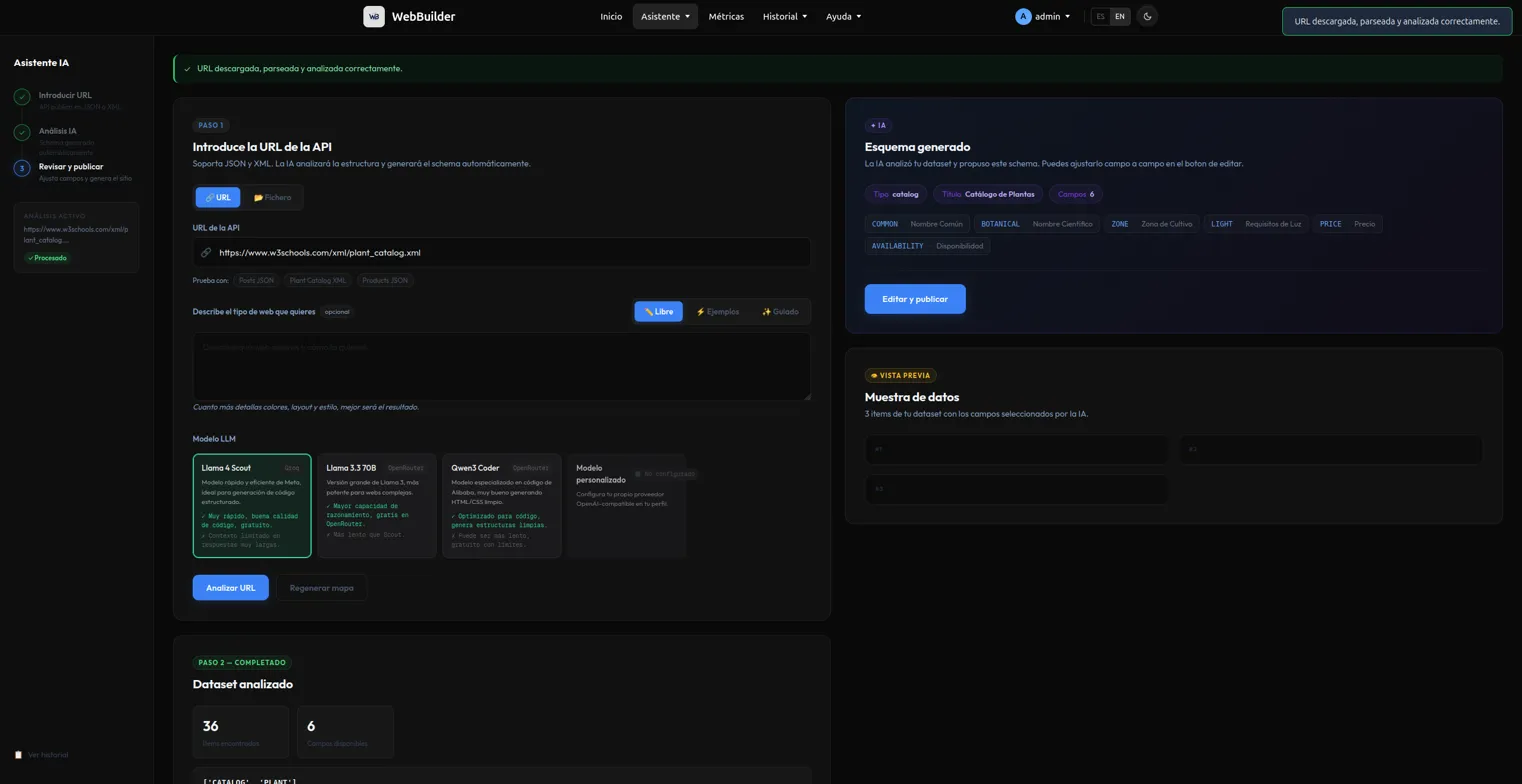
\includegraphics[width=\textwidth]{img/oldversions/previewold.png}
    \caption{Interfaz del asistente tras el refactor visual del Sprint 5}
    \label{fig:previewold}
\end{figure}

\subsection{Enriquecimiento de prompts}
\label{subsec:enriquecimiento-prompts}

Tras unas cuantas pruebas, se llegó a la conclusión de un problema importante, podría ocurrir que un usuario no familiarizado con los prompts de IA no supiese cómo hacerlo adecuadamente, o que incluso lo dejase vació. Para resolver este problema se creó el fichero \texttt{utils/llm/enrich\_prompts.py}, 
encargado de analizar automáticamente los campos del dataset antes de construir el prompt y añadir contenido personalizado.
Si el dataset tenía campos con imagenes se le indica al modelo que las usara de forma destacada. Si tenía precios, que los resalte visualmente. Si tenía
fechas que las mostrara de forma clara. De esta forma se garantiza que el LLM siempre recibiera suficiente contexto para tomar decisiones razonadas.
De todos modos si algo no estuviese en la mente del usuario, en el siguiente paso de editar el schema podría modificarlo añadiendo los campos necesarios o modificando los existentes.


\subsection{Trazabilidad: GenerationLog}
\label{subsec:trazabilidad-generationlog}

Anteriormente en las generaciones si algo fallaba no había forma de saber qué prompt se había enviado exactamente, qué había respondido el modelo ni si había habido reintentos. Para arreglar esto se creó el modelo \textbf{GenerationLog}, vinculado mediante una clave a su correspondiente \textbf{GeneratedSite}. 

Cada llamada al LLM durante la generación de un proyecto producía un registro que almacenaba el paso concreto que se estaba generando, el modelo de LLM utilizado, el prompt de sistema y el prompt de usuario enviados, la respuesta en crudo devuelta por el modelo, los errores de consistencia detectados y si la llamada había necesitado un reintento. Esto permitía analizar a posteriori qué pasos fallaban con más frecuencia, qué modelos producían mejores resultados y qué tipos de datasets generaban más inconsistencias.


\subsection{Verificación de consistencia}
\label{subsec:verificacion-consistencia}

Otro problema frecuente era que el LLM no tenía suficiente contexto entre ficheros, principal causa de las alucinaciones del LLM. Ocurria lo siguiente:
se definía un campo con un nombre en \textbf{models.py} y luego en los demás ficheros se referenciaba con ligeros cambios, provocando errores de ejecución.
Para detectar estos casos antes de que el usuario desplegase el proyecto, se implementó el fichero \texttt{utils/llm/consistency\_checker.py}.

Este fichero extraía mediante expresiones regulares los campos definidos en \texttt{models.py} y buscaba en los demas templates las referencias a esos campos. Cualquier referencia encontrada diferente que no correspondiera al campo real del modelo, se registraba como error de consistencia. 
Estos errores se guardaban en el campo \texttt{consistency\_errors} del modelo \texttt{GenerationLog} correspondiente, permitiendo identificar qué pasos producian mas inconsistencias y cómo se producían, para el consiguiente arreglo a futuro.


\subsection{Panel de métricas}
\label{subsec:panel-metricas}

Para tener un uso mas sencillo y accesible del contenido de GenerationLog se añadió una vista de métricas en \textbf{views/metrics.py}, accesible únicamente para usuarios con permisos de administrador. El objetivo de esta vista era tener visibilidad real sobre el comportamiento del generador, los fallos más recurrentes, qué modelos eran más óptimos para cada tipo de página, etc.

El panel mostraba las siguientes estadísticas agregadas:

\begin{itemize}
    \item \textbf{Resumen general}: número total de registros en \texttt{GenerationLog}, sitios generados y análisis realizados hasta la fecha.
    \item \textbf{Desglose por paso}: para cada uno de los siete pasos del generador, se mostraba el número de llamadas realizadas, cuántas habían necesitado reintento y la tasa de reintento resultante. Esto permitía identificar qué pasos eran más problemáticos y priorizar las mejoras.
    \item \textbf{Distribución por modelo}: agrupación de las llamadas por modelo de LLM utilizado, lo que facilitaba comparar el rendimiento de distintos proveedores cuando se probaban configuraciones diferentes.
\end{itemize}

Esta información resultó útil para mejorar los siguientes sprints y realizar los cambios adecuados. Los datos reales recogidos por este panel se analizan en detalle en la Sección~\ref{sec:metricas-sistema}.

